  
\documentclass{beamer} 
 \usepackage{beamerthemedefault, multimedia} 
 \useoutertheme{smoothbars} 
 \useinnertheme[shadow=true]{rounded} 
 \setbeamercovered{transparent} 
 \setbeamertemplate{navigation symbols}{} 
 \setbeamertemplate{footline}[frame number] 
\usepackage{graphicx} 
\usepackage{morefloats} 
\usepackage{amsmath} 
\usepackage{amssymb} 
\usepackage{rotating} 
% mcode options for matlab code insertion bw (for printing), numbered (line numbers), framed (frame around code blocks), useliterate (convert Matlab expressions to Latex ones), autolinebreaks (automatic code wraping, use it with caution 
\usepackage[literate]{mcode} 
\graphicspath{{figures/}{tex/}{../figures/}{../../}{../}}  
\title{timbralSimilaritySolScatteringTechniqueSlides} 
\author{ Mathieu Lagrange } 
  
\begin{document} 
  
\maketitle 
  
% Please use this file to document your experiment 
% You can compile the report by setting the option 'report' as detailed in your expLanes configuration file. 
  
This is the report to document the expLanes project timbralSimilaritySol using \LaTeX. 
  
  
 
  
  
\begin{frame}\frametitle{Factors flow graph} 
  
  
\begin{center} 
  
  
\begin{figure} 
  
  
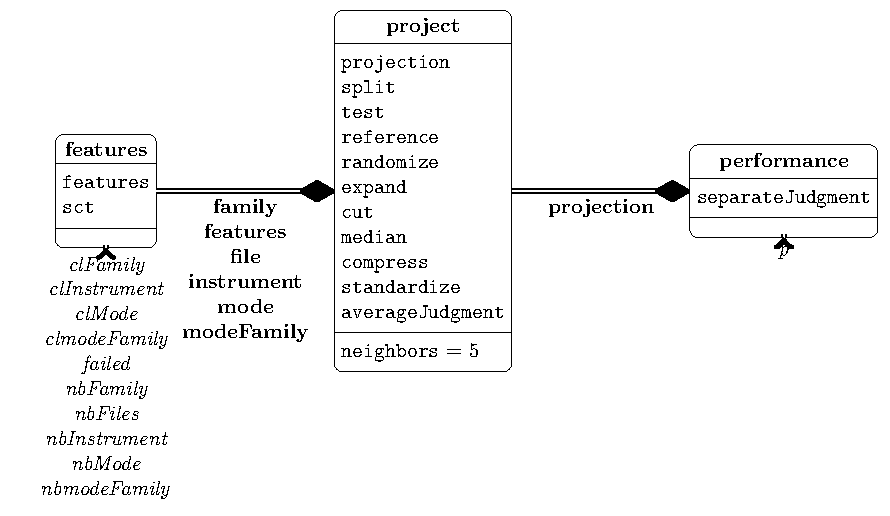
\includegraphics[width=\textwidth,height=0.8\textheight,keepaspectratio]{../figures/factors.pdf} 
  
  
\label{factorFlowGraph} 
  
  
\end{figure} 
  
  
\end{center} 
  
  
\end{frame} 
  
\begin{frame}\frametitle{sct: 25, projection: lmnn, split: none, reference: judgments, randomize: 0, expand: 0, cut: 1, median: 1, compress: 1, standardize: 1, averageJudgment: 0} 
  
\begin{table} 
\begin{center} 
\ 
 \setlength{\tabcolsep}{.16667em} 
\begin{tabular}{llc} 
fea & sepjud & p (\%) \\ 
\hline 
mfcc & 0 & 86.3 \\ 
mfcc & 1 & 86.2 \\ 
mfcc & 2 & 85.1 \\ 
scat & 0 & 91.6 \\ 
scat & 1 & 95.2 \\ 
scat & 2 & 86.4 \\ 
tfscat & 0 & \textbf{96.2} \\ 
tfscat & 1 & \textbf{\textcolor{red}{96.9}} \\ 
tfscat & 2 & 91.1 \\ 
\end{tabular} 
\end{center} 
\label{sc25PrlmSpnoRejuRa0Ex0Cu1Me1Co1St1Avju0} 
\end{table} 
 
\end{frame}  
 % expLanesInsertionFlag DO NOT CLEAR (but move it where you want the generated temporary LaTEX code to be inserted) 
  
  
\bibliographystyle{abbrvnat} 
\bibliography{bib} 
  
\end{document} 
